% \documentclass[draft,11pt]{article}
%\documentclass[11pt]{article}
\chapter{Classical
  Algorithms for Maximum Flow I}
\label{cha:maxflow1}
%%  RASMUS  packages
\usepackage{blindtext}
\usepackage[usenames,dvipsnames,svgnames,table]{xcolor}
\usepackage{enumitem}
\usepackage{caption}
\usepackage{placeins}
\usepackage{graphicx}

\usepackage{fancybox}
\usepackage{hyperref}

\usepackage{amsmath,amsfonts,amsthm,amssymb,xcolor}
% \let\amsboldsymbol\boldsymbol % if you want to see the bad
% boldsymbol for comparison
\usepackage{bm} % fixes boldsymbol

\usepackage{nicefrac}

\usepackage{float}


% switched to algorithm2e in lecture 9
% \usepackage{algorithm} %ctan.org\pkg\algorithms
% \usepackage{algorithmic}
% \usepackage{algorithmicx}
% \usepackage[noend]{algpseudocode}

\newtheorem{theorem}{Theorem}[section]
\newtheorem{corollary}[theorem]{Corollary}
\newtheorem{lemma}[theorem]{Lemma}
\newtheorem{observation}[theorem]{Observation}
\newtheorem{proposition}[theorem]{Proposition}
\newtheorem{claim}[theorem]{Claim}
\newtheorem{fact}[theorem]{Fact}
\newtheorem{assumption}[theorem]{Assumption}
\newtheorem{warning}[theorem]{Warning}
\newtheorem{conjecture}[theorem]{Conjecture}

\theoremstyle{definition}
\newtheorem{definition}[theorem]{Definition}
\newtheorem{remark}[theorem]{Remark}

\newtheorem*{theorem*}{Theorem}
\newtheorem*{corollary*}{Corollary}
\newtheorem*{conjecture*}{Conjecture}
\newtheorem*{lemma*}{Lemma}
\newtheorem*{thm*}{Theorem}
\newtheorem*{prop*}{Proposition}
\newtheorem*{obs*}{Observation}
\newtheorem*{definition*}{Definition}
\newtheorem*{example}{Example}
\newtheorem*{remark*}{Remark}
\newtheorem*{rec*}{Recommendation}

\newenvironment{fminipage}%
  {\begin{Sbox}\begin{minipage}}%
  {\end{minipage}\end{Sbox}\fbox{\TheSbox}}

\newenvironment{algbox}[0]{\vskip 0.2in
\noindent 
\begin{fminipage}{6.3in}
}{
\end{fminipage}
\vskip 0.2in
}


\let\muchl\ll

\def\pleq{\preccurlyeq}
\def\pgeq{\succcurlyeq}
\def\pge{\succ}
\def\ple{\prec}

\def\Approx#1{\approx_{#1}}

%\def\Span#1{\textbf{Span}\left(#1  \right)}
\def\bvec#1{{\mbox{\boldmath $#1$}}}




\def\prob#1#2{\mbox{Pr}_{#1}\left[ #2 \right]}
\def\pvec#1#2{\vec{\mbox{P}}^{#1}\left[ #2 \right]}
\def\expec#1#2{{\mathbb{E}}_{#1}\left[ #2 \right]}
\def\var#1{\mbox{\bf Var}\left[ #1 \right]}

\def\defeq{\stackrel{\mathrm{def}}{=}}
\def\setof#1{\left\{#1  \right\}}
\def\sizeof#1{\left|#1  \right|}


\def\trace#1{\mathrm{Tr} \left(#1 \right)}

\def\floor#1{\left\lfloor #1 \right\rfloor}
\def\ceil#1{\left\lceil #1 \right\rceil}

\def\dim#1{\mathrm{dim} (#1)}
\def\sgn#1{\mathrm{sgn} (#1)}

\def\union{\cup}
\def\intersect{\cap}
\def\Union{\bigcup}
\def\Intersect{\bigcap}

\def\abs#1{\left|#1  \right|}

\def\norm#1{\left\| #1 \right\|}
\def\smallnorm#1{\| #1 \|}

\newcommand\grad{\boldsymbol{\nabla}}
\newcommand\D[2]{D#1[#2]}

\newcommand*\diff{\mathop{}\!\mathrm{d}}
\newcommand*\Diff[1]{\mathop{}\!\mathrm{d^#1}}

\newcommand\ip[1]{\left< #1 \right>}


\newcommand{\sym}[1]{\mathrm{sym} (#1)}



\def\calC{\mathcal{C}}
\def\calD{\mathcal{D}}
\def\calE{\mathcal{E}}
\def\calF{\mathcal{F}}
\def\calG{\mathcal{G}}
\def\calL{\mathcal{L}}
\def\calS{\mathcal{S}}
\def\calT{\mathcal{T}}
\def\calM{\mathcal{M}}

\newcommand\calDD{\boldsymbol{\calD}}

\newcommand\DDelta{\boldsymbol{\mathit{\Delta}}}
\newcommand\Ppsi{\boldsymbol{\mathit{\Psi}}}
\newcommand\PPsi{\boldsymbol{\mathit{\Psi}}}
\newcommand\ppsi{\boldsymbol{\mathit{\psi}}}
\newcommand\pphi{\boldsymbol{\mathit{\phi}}}
\newcommand\PPhi{\boldsymbol{\Phi}}
%\newcommand\Llambda{\boldsymbol{\mathit{\Lambda}}}
\newcommand\LLambda{\boldsymbol{\mathit{\Lambda}}}
\newcommand\PPi{\boldsymbol{\Pi}}

\newcommand\ppi{\boldsymbol{\pi}}
\newcommand\cchi{\boldsymbol{\chi}}
\newcommand\aalpha{\boldsymbol{\alpha}}
\newcommand\bbeta{\boldsymbol{\beta}}
\newcommand\ggamma{\boldsymbol{\gamma}}
\newcommand\ddelta{\boldsymbol{\delta}}

\newcommand\rrho{\boldsymbol{\rho}}
\newcommand\xxi{\boldsymbol{\xi}}
%\newcommand\cchi{\boldsymbol{\chi}}

\newcommand\er{R_{\text{eff}}}


\def\aa{\pmb{\mathit{a}}}
\newcommand\bb{\boldsymbol{\mathit{b}}}
\newcommand\cc{\boldsymbol{\mathit{c}}}
\newcommand\dd{\boldsymbol{\mathit{d}}}
\newcommand\ee{\boldsymbol{\mathit{e}}}
\newcommand\ff{\boldsymbol{\mathit{f}}}
\renewcommand\gg{\boldsymbol{\mathit{g}}}
\newcommand\ii{\boldsymbol{\mathit{i}}}
\newcommand\jj{\boldsymbol{\mathit{j}}}
\newcommand\kk{\boldsymbol{\mathit{k}}}
\renewcommand\ll{\boldsymbol{\mathit{l}}}
\newcommand\pp{\boldsymbol{\mathit{p}}}
\newcommand\qq{\boldsymbol{\mathit{q}}}
\newcommand\bs{\boldsymbol{\mathit{s}}}
\newcommand\nn{\boldsymbol{\mathit{n}}}
\newcommand\rr{\boldsymbol{\mathit{r}}}
\renewcommand\ss{\boldsymbol{\mathit{s}}}
\def\tt{\boldsymbol{\mathit{t}}}
\newcommand\uu{\boldsymbol{\mathit{u}}}
\newcommand\vv{\boldsymbol{\mathit{v}}}
\newcommand\ww{\boldsymbol{\mathit{w}}}
\newcommand\yy{\boldsymbol{\mathit{y}}}
\newcommand\zz{\boldsymbol{\mathit{z}}}
\newcommand\xx{\boldsymbol{\mathit{x}}}

\newcommand\veczero{\boldsymbol{0}}
\newcommand\vecone{\boldsymbol{1}}

\newcommand\matzero{\boldsymbol{0}}
\newcommand\matone{\boldsymbol{1}}

\newcommand{\matlow}{\boldsymbol{\mathit{{\mathcal{L}}}}}
\newcommand{\matlowtil}{\boldsymbol{\mathit{\widetilde{\mathcal{L}}}}}
\newcommand{\matlowhat}{\boldsymbol{\mathit{\widehat{\mathcal{L}}}}}

\newcommand{\matup}{\boldsymbol{\mathit{{\mathcal{U}}}}}


\renewcommand\AA{\boldsymbol{\mathit{A}}}
\newcommand\BB{\boldsymbol{\mathit{B}}}
\newcommand\CC{\boldsymbol{\mathit{C}}}
\newcommand\DD{\boldsymbol{\mathit{D}}}
\newcommand\EE{\boldsymbol{\mathit{E}}}
\newcommand\GG{\boldsymbol{\mathit{G}}}
\newcommand\HH{\boldsymbol{{H}}}
\newcommand\II{\boldsymbol{\mathit{I}}}
\newcommand\JJ{\boldsymbol{\mathit{J}}}
\newcommand\KK{\boldsymbol{\mathit{K}}}
\newcommand\NN{\boldsymbol{\mathit{N}}}
\newcommand\MM{\boldsymbol{\mathit{M}}}
\newcommand\LL{\boldsymbol{\mathit{L}}}
\newcommand\PP{\boldsymbol{\mathit{P}}}
\newcommand\RR{\boldsymbol{\mathit{R}}}
\renewcommand\SS{\boldsymbol{\mathit{S}}}
\newcommand\TT{\boldsymbol{\mathit{T}}}
\newcommand\UU{\boldsymbol{\mathit{U}}}
\newcommand\WW{\boldsymbol{\mathit{W}}}
\newcommand\VV{\boldsymbol{\mathit{V}}}
\newcommand\XX{\boldsymbol{\mathit{X}}}
\newcommand\YY{\boldsymbol{\mathit{Y}}}



\newcommand\MMtil{\boldsymbol{\mathit{\tilde{M}}}}
\newcommand\AAtil{\boldsymbol{\mathit{\tilde{A}}}}
\newcommand\BBtil{\boldsymbol{\mathit{\tilde{B}}}}
\newcommand\LLtil{\boldsymbol{\mathit{\tilde{L}}}}
\newcommand\MMtilde{\boldsymbol{\mathit{\tilde{M}}}}
\newcommand\XXtil{\boldsymbol{\mathit{\tilde{X}}}}

\newcommand\AAn{\boldsymbol{\mathcal{A}}}
\newcommand\ZZ{\boldsymbol{\mathit{Z}}}

\newcommand\AAhat{\boldsymbol{\widehat{\mathit{A}}}}
\newcommand\AAapprox{\boldsymbol{\widetilde{\mathit{A}}}}
\newcommand\DDhat{\boldsymbol{\widehat{\mathit{D}}}}
\newcommand\DDapprox{\boldsymbol{\widetilde{\mathit{D}}}}
\newcommand\LLhat{\boldsymbol{\widehat{\mathit{L}}}}
\newcommand\LLapprox{\boldsymbol{\widetilde{\mathit{L}}}}
\newcommand\MMhat{\boldsymbol{\widehat{\mathit{M}}}}
\newcommand\MMapprox{\boldsymbol{\widetilde{\mathit{M}}}}
\newcommand\ZZhat{\boldsymbol{\widehat{\mathit{Z}}}}

\newcommand\DDtil{\boldsymbol{\widetilde{\mathit{D}}}}

\newcommand\fftil{\boldsymbol{\tilde{\mathit{f}}}}
\newcommand\sstil{\boldsymbol{\tilde{\mathit{s}}}}
\newcommand\xxtil{\boldsymbol{\tilde{\mathit{x}}}}
\newcommand\yytil{\boldsymbol{\tilde{\mathit{y}}}}
\newcommand\wwtil{\boldsymbol{\tilde{\mathit{w}}}}


\newcommand\Otil{\widetilde{O}}

\newcommand\xhat{{\hat{{x}}}}
\newcommand\uhat{{\hat{{u}}}}
\newcommand\uuhat{\boldsymbol{\mathit{\hat{u}}}}
\newcommand\vhat{{\hat{{v}}}}
\newcommand\what{{\hat{{w}}}}

\newcommand\Ghat{{\widehat{{G}}}}
\newcommand\GGhat{\boldsymbol{\widehat{G}}}

\newcommand\R{\mathbb{R}}
\newcommand\N{\mathbb{N}}

\newcommand\ffhat{\boldsymbol{\hat{\mathit{f}}}}

\newcommand\cchat{\boldsymbol{\widehat{\mathit{c}}}}
\newcommand\sshat{\boldsymbol{\mathit{\widehat{s}}}}
\newcommand\xxhat{\boldsymbol{\mathit{\widehat{x}}}}
\newcommand\yyhat{\boldsymbol{\widehat{\mathit{y}}}}
\newcommand\xxbar{\overline{\boldsymbol{\mathit{x}}}}
\newcommand\yybar{\overline{\boldsymbol{\mathit{y}}}}
\newcommand\xxstar{{\boldsymbol{\mathit{x}}^{*}}}
\newcommand\yystar{{\boldsymbol{\mathit{y}}^{*}}}


\newcommand\ffbar{\overline{\boldsymbol{\mathit{f}}}}


\newcommand\energy{\mathcal{E}}


\newcommand{\todo}[1]{{\bf \color{red} TODO: #1}}
\newcommand{\todolow}[1]{{\bf \color{orange} TODOLOW: #1}}

\newcommand{\richard}[1]{{\bf \color{green} Richard: #1}}
\newcommand{\rasmus}[1]{{\bf \color{olive} Rasmus: #1}}
\newcommand{\ahad}[1]{{\bf \color{olive} Ahad: #1}}


\newcommand{\expct}[2]{{}\mathop{\mathbb{E}}_{#1}\left[#2\right]}
\newcommand{\E}[1]{\mathop{{}\mathbb{E}}\left[#1\right]}
%% https://tex.stackexchange.com/questions/56765/getting-the-expectation-symbol-to-behave-like-sum-instead-of-sigma
%% extra {} inside mathop gives nicer (standard) vertical placement of E
\newcommand{\Var}[1]{\mathop{{}Var}\left[#1\right]}
\newcommand{\Ex}[1]{{}\mathop{\mathbb{E}}_{#1}}
\newcommand\tr{\mathrm{Tr}}


%%%%% LINEAR ALGEBRA

\newcommand{\schurto}[2]{\ensuremath{\textsc{Sc}\!\left[#1\right]_{#2}}}
% \newcommand{\schurto}[2]{\ensuremath{\textsc{Sc}\left[#1\right]_{#2}}}

%{$\textsc{Sc}\left[#1\right]_{#2}$}
% \newcommand{\schurto}[2]{\textsc{Sc}\left(#1, #2\right)}
%\newcommand{\schurto}[2]{\left[{#1}\right]_{\to #2}}
\renewcommand{\sc}[2]{\schurto{#1}{#2}}

%transpose
\newcommand{\trp}{\top}

%pseudoinverse
\newcommand{\pinv}{+}


\newcommand{\proj}{\PPi}

\DeclareMathOperator{\nnz}{nnz}

\DeclareMathOperator*{\argmin}{arg\,min}
\DeclareMathOperator*{\argmax}{arg\,max}
\DeclareMathOperator*{\val}{val}

\DeclareMathOperator*{\diag}{diag}
\DeclareMathOperator*{\Span}{span}

%\DeclareMathOperator*{\ker}{ker}
\DeclareMathOperator*{\im}{im}

%%%%% LAYOUT

\newenvironment{tight_enumerate}{
\begin{enumerate}
 \setlength{\itemsep}{2pt}
 \setlength{\parskip}{1pt}
}{\end{enumerate}}
\newenvironment{tight_itemize}{
\begin{itemize}
 \setlength{\itemsep}{2pt}
 \setlength{\parskip}{1pt}
}{\end{itemize}}
\newenvironment{tight_description}{
\begin{description}
 \setlength{\itemsep}{2pt}
 \setlength{\parskip}{1pt}
}{\end{description}}

\newcommand*{\vertbar}{\rule[-1ex]{0.5pt}{2.5ex}}
\newcommand*{\horzbar}{\rule[.5ex]{2.5ex}{0.5pt}}

%Basics
\newcommand{\new}[1]{{\em #1\/}}		% New term (set in italics).

\newcommand{\boxwidth}{\dimexpr\linewidth-2em\relax}

\newcommand{\boxdef}[1]
{
\fbox{
\begin{minipage}{\boxwidth}
\begin{definition}
{#1}
\end{definition}
\end{minipage}
}
}

\newcommand{\boxthm}[1]
{
\fbox{
\begin{minipage}{\boxwidth}
\begin{theorem}
{#1}
\end{theorem}
\end{minipage}
}
}

\newcommand{\boxfact}[1]
{
\fbox{
\begin{minipage}{\boxwidth}
%\begin{theorem*}
\emph{{#1}
%\end{theorem*}
}
\end{minipage}
}
}

%\newcommand{\handout}[5]{
  \noindent
  \begin{center}
  \framebox{
    \vbox{
            \hbox to 6.30in { {\bf Advanced Graph Algorithms and Optimization} \hfill #2 }
            \vspace{5mm}
            \hbox to 6.30in { {\Large \hfill #5  \hfill} }
            \vspace{3mm}
            \hbox to 6.30in { {\em #3 \hfill #4} }
    }
  }
  \end{center}
  \vspace*{4mm}
}

\newcommand{\lecture}[4]{\handout{#1}{#2}{#3}{Lecture #1}{#4}}
\newcommand{\homework}[3]{\handout{#1}{#2}{#3}{Problem Set #1}}
\newcommand{\gradedhomework}[3]{\handout{#1}{#2}{#3}{Graded Homework #1}}
\newcommand{\sect}[3]{\handout{#1}{#2}{#3}{Section #1}}




% 1-inch margins, from fullpage.sty by H.Partl, Version 2, Dec. 15, 1988.
\topmargin 0pt
\advance \topmargin by -\headheight
\advance \topmargin by -\headsep
\textheight 8.9in
\oddsidemargin 0pt
\evensidemargin \oddsidemargin
\marginparwidth 0.5in
\textwidth 6.5in

\parindent 0in
\parskip 1.5ex
 
%\usepackage{amsmath}
%\usepackage{amssymb}
%\usepackage{amsthm}
%\usepackage{graphicx}
%\usepackage{float}
%\usepackage[ruled,vlined]{algorithm2e}
%\SetKwBlock{Repeat}{repeat}{}
%%% for this lecture
%\newcommand{\gap}{\text{gap}}
% \newtheorem{theorem}{Definition}
%\interfootnotelinepenalty=10000
% \newtheorem{lemma}{Lemma}


%\begin{document}

\sloppy
%\lecture{10 --- Wednesday, April 29th}
%{Spring 2020}{Rasmus Kyng, Scribe: Meher Chaitanya}{Classical
  %Algorithms for Maximum Flow}
\section{Maximum Flow}
% \section{Overview}
In this chapter, we will study the \emph{Maximum Flow Problem} and
    discuss some classical algorithms for finding solutions to it.
% Talk about max flow, classical algorithms for maximum
% flow. interesting open problems with things we can do with classical
% algorithms and things we can do with modern algorithms and close the
% gap between them.
% 
\paragraph{Setup.} Consider a directed graph \(G=(V, E, \cc)\), where
$V$ denotes vertices, $E$ denotes edges and $\cc \in \R^{E},  \cc \geq 0$ denotes edge
capacities. In contrast to earlier chapters, the direction
of each edge will be important, and not just as a book keeping tool
(which is how we previously used it in undirected graphs).
We consider an edge $(u,v) \in E$ to be \emph{from} $u$ and \emph{to}
$v$.
Edge capacities are associated with directed edges, and we allow both
edge $(u,v)$ and $(v,u)$ to exist, and they may have different
capacities.

A \emph{flow} is any vector $\ff \in \R^E.$

We say that a flow is feasible
when $\veczero \leq \ff \leq \cc$.
The constraint $\veczero \leq \ff$ ensures that the flow respects edge
directions, while the constraint $\ff \leq \cc$ ensures that the flow
does not exceed capacity on any edge.

We still define the edge-vertex incidence matrix $\BB \in \R^{V \times E}$ of $G$ by
\[
  \BB(v,e) =
  \begin{cases}
    1 & \text{ if } e = (u,v) \\
    -1 &\text{ if } e = (v,u) \\
    0 &\text{ o.w.}
  \end{cases}
\]
As in the undirected case, a \emph{demand vector} is a vector \(\dd \in \R^{V} \).
And as in the undirected case, we can express the net flow constraint that
$\ff$ routes the demand $\dd$ by
\[
  \BB \ff = \dd
  .
\]
We will focus on the case:
  \begin{equation} \nonumber
      \BB\ff= F (-\ee_{s}+\ee_t) = F \bb_{st}.
  \end{equation}
 Flows that satisfy the above equation for some scalar \(F\) are
 called $s$-$t$ flows where \(s, t \in V\).
 The vertex \(s\) is called the source, \(t\) is called the sink and  \(\ee_s\), \(\ee_t\) are indicator vectors for source and sink nodes respectively. The vector \(\bb_{st}\) has -1 at source and 1 at sink. The maximum flow can be expressed as a linear program as follows
 \begin{equation}
   \label{eq:maxflow}
\begin{aligned}
\max_{\ff \in \R^E,F} \quad & F\\
\textrm{s.t.} \quad & \BB\ff= F \bb_{st}\\
  & 0 \leq \ff \leq \cc   \\
\end{aligned}
\end{equation}
We use $\val(\ff)$ to denote $F$ when $B\ff = F\bb_{st}$.


\section{Flow Decomposition}
We now look at a way of simplifying flows
\begin{definition}
  A $s$-$t$ path flow is a flow \(\ff \geq \veczero\) that can be written as
  \begin{equation}\nonumber
      \ff = \alpha \sum_{e \in p} \ee_e
  \end{equation}
  where p is a simple path from s to t.
\end{definition}
\begin{definition}
  A cycle flow is a flow \(\ff \geq \veczero \) that can be written as a cycle i.e.
  \begin{equation}\nonumber
      \ff = \alpha \sum_{e \in c} \ee_e
  \end{equation}
  where c is a simple cycle.
\end{definition}
% }
% \item GRADED? gaussian elimination for Laplacians is closed ?
% \end{enumerate}
\begin{lemma}[The path-cycle decomposition lemma]
 Any $s$-$t$ flow \(\ff\) can be decomposed into a sum of $s$-$t$ path
 flows and cycle flows such that the sum contains at most
 \(\nnz(\ff)\) terms. Note $\nnz(\ff) \leq \abs{E}$.
\end{lemma}
\begin{proof}
We perform induction on the number of edges with non-zero flow, which
we denote by $\nnz(\ff)$.
Note that by ``the support of $\ff$'', we mean the set $\setof{e \in E :
  \ff(e) \neq 0}$.
\paragraph{Base case:}  \(\ff = 0\): nothing to do.
\paragraph{Inductive step:}
Try to find a path from \(s\) to \(t\) OR a cycle in the support of \(\ff\). \\
\emph{``Path'' case.}
If there exists such a $s$-$t$ path, let \(\alpha\) be the minimum flow value along the edges of the path, i.e.
\begin{equation} \nonumber
\begin{aligned}
\alpha = \min_{(a,b) \in p} \ff(a,b)
\end{aligned}
\end{equation}
\begin{equation} \nonumber
    \ff^{'} = \alpha \sum_{e \in p} \ee_e
\end{equation}
Update the flow $\ff$ by
\begin{equation} \nonumber
    \ff  \leftarrow \ff - \ff'
\end{equation}
The value of the flow will still be non-negative after this update as we
subtracted the minimum entry along any positive edge on the path. The
number of non-zeros, $\nnz(\ff)$, went down by at least one.
Note that the updated $\ff$ must again be an $s$-$t$ flow, as it is the
difference of two $s$-$t$ flows.
% If we continue this procedure by finding paths,
% eventually the flow value $\val(\ff)$ must become zero.

\emph{``Cycle'' case.}
Suppose we find a cycle \(c\) in the support of \(\ff\).
Let \(\alpha\) be the minimum flow value along the edges of the cycle, i.e.\
\begin{equation*}
\alpha = \min_{(a,b) \in c} \ff(a,b)
\end{equation*}
\begin{equation*}
 \ff^{'} = \alpha \sum_{e \in c} \ee_e
\end{equation*}
Update the flow $\ff$ by
\begin{equation} \nonumber
    \ff  \leftarrow \ff - \ff'
  \end{equation}
  As in the path case, $\ff$ stays non-negative, and
number of non-zeros, $\nnz(\ff)$, goes down by at least one.
Note that the updated $\ff$ must again be an $s$-$t$ flow, as it is the
difference of two $s$-$t$ flows.

\emph{``No path or cycle'' case.}
Suppose we can find neither a path nor a cycle, and $\ff \neq
\veczero$.
Then there must be an edge $(u,v)$ with non-zero flow leading into a
vertex $v \neq s,t$ and with no outgoing edge from
$v$ in the support of $\ff$.
In that case, we must have $(\BB\ff)(v) \geq 0$.
But since $v \neq t$, this contradicts $\BB \ff = F \bb_{st} $.
So this case cannot occur.
\end{proof}
\begin{lemma}
In any $s$-$t$ max flow problem instance, there is an optimal flow \(\ff^*\) with a path-cycle decomposition that has only paths and no cycles.
\end{lemma}

\begin{proof} Let \(\fftil\) be an optimal flow. Let \(\ff^*\) be the
  sum of path flows in the path cycle decomposition of
  \(\fftil\). They route the same flow (as cycles contribute to no net
  flow from $s$ to $t$). Thus
 \begin{align*}
  \BB\ff^* = \BB\fftil
 \end{align*}
 and hence $\val(\ff^*) = \val(\fftil)$.
 Furthermore
\begin{equation*}
  \veczero \leq \ff^* \leq \fftil \leq \cc
\end{equation*}
The first inequality follows from  \(\ff^*\) being a sum of positive
path flow.
The second inequality holds as $\ff^*$ is upper bounded in every single entry by \(\fftil\), because we reduced
it by positive entry cycles.
The third inequality holds because
$\fftil$ is a feasible flow, so it is upper bounded by the capacities.
\end{proof}
An optimal flow solving the maximum flow problem may not be unique.
For example, consider the graph below with source s and sink t:\\
\begin{figure}[H]
 \centering
  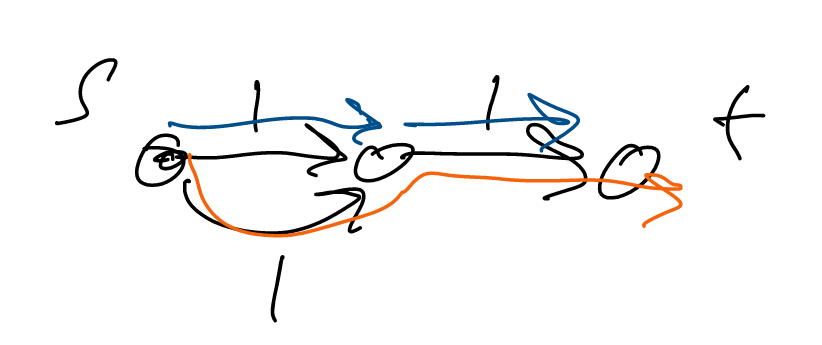
\includegraphics[width=50mm,scale=0.1]{fig/fig1_lec10.PNG}
  \label{fig:ex1}
\end{figure}
There are two optimal paths in this example.
Maximum flow is a convex optimization problem but not a strongly
convex problem as the solutions are not unique, and this is part of
what makes it hard to solve.

\section{Cuts and Minimum Cuts}

The decomposition shown earlier provides a way to show that the
maximum flow in a graph is upper bounded by constructing graph
cuts.

Given a vertex subset $S \subseteq V$, we say that $(S, V\setminus S)$
is a \emph{cut} in $G$ and that the value of the cut is
\[
  c_G(S) = \sum_{e \in E \intersect (S \times V\setminus S) } \ww(e)
  .
\]

Note that in a directed graph, only edges crossing the cut
going \emph{from} $S$ and \emph{to} $V\setminus S$ count toward the cut.

\begin{figure}[H]
 \centering
 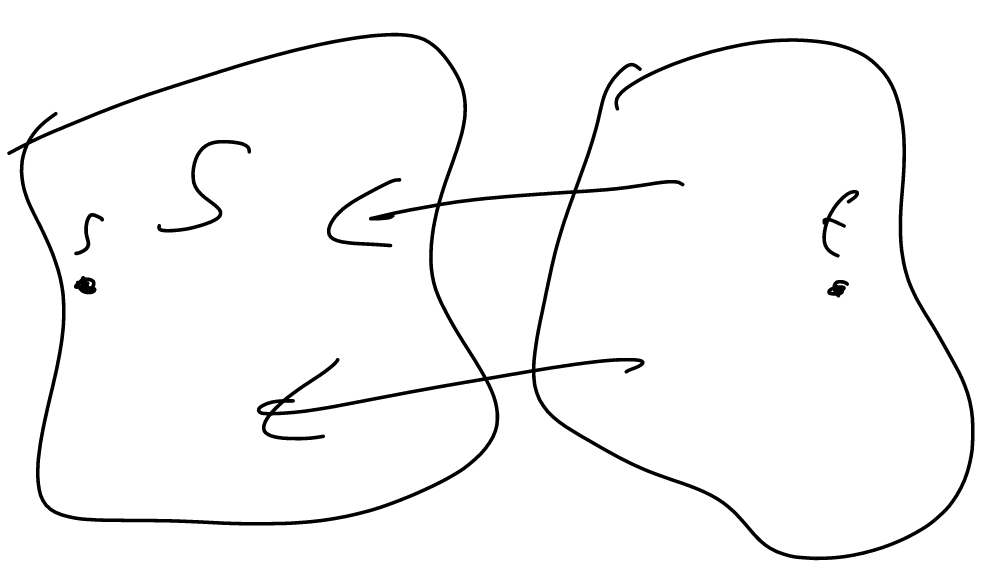
\includegraphics[width=50mm,scale=0.1]{fig/fig2_lec10.PNG}
 \caption{Example of a cut: No edges go from $S$ to $(S, V\setminus
   S)$, and so the value of this cut is zero.}
  \label{fig:cutnoforwardedges}
\end{figure}

\begin{definition*}
  ($s$-$t$ cuts). We define an $s$-$t$ cut to be a subset $S \subset
  V$, where $s \in S$ and $t \in V \setminus S$.


  %\begin{equation}\nonumber
  %    \ff = \alpha \sum_{e \in c} %\underline{e}_{e}
 % \end{equation}
  %where c is a simple cycle.
\end{definition*}

\paragraph{A decision problem:}
\emph{``Given an instance of the Maximum Flow  problem, is there a flow from s to t such that \(\ff \neq \veczero\)?''}

\begin{description}
\item[If YES:] We can decompose this flow into $s$-$t$ path flows and
  cycle flows.
\item[If NO:]  There is no flow path from $s$ to $t$. Let $S$ be the
  set of vertices reachable from source $s$. Then (\(S,V \setminus
  S\)) is a cut in the graph, with no edges crossing from $S$ to \( V
  \setminus S\). Figure~\ref{fig:cutnoforwardedges} gives an example.
\end{description}

\paragraph{Upper bounding the maximum possible flow value.}
How can we recognize a maximum flow? Is there a way to confirm that a
flow is of maximum value?

We can now introduce the \emph{Minimum Cut} problem.
%
\begin{align}
   \label{eq:mincutset}
\min_{S \subseteq V } \ & c_G(S)\\ \nonumber
\textrm{s.t. } & s \in V \text{ and } t \not\in V
\end{align}
The Minimum Cut problem can also be phrased as a linear program,
although we won't see that today.

We'd like to obtain a tight connection between flows and cuts in the
graph.
As a first step, we won't get that, but we can at least observe that the value of any $s$-$t$ cut
provides an upper bound to the maximum possible $s$-$t$ flow value.

\begin{theorem}[Max Flow $\leq$ Min Cut] The maximum $s$-$t$ flow
  value in a directed graph G \mbox{(Program~\eqref{eq:maxflow})} is upper bounded by the minimum value of
  any $s$-$t$ cut (Program~\eqref{eq:mincutset}).
  I.e.\ if $S$ is an $s$-$t$ cut, and $\ff$ a feasible $s$-$t$ flow
  then
  \[
    \val(\ff) \leq c_G(S)
  \]
  And in particular this holds for any minimum cut $S^*$ and maximum
  flow $\ff^*$, i.e.\
  $\val(\ff^*) \leq c_G(S^*)$.
\end{theorem}
\begin{proof}


Consider any feasible flow  \(0 \leq \ff \leq \cc \) and a cut \(S,T = V\setminus S\).
% such that \(S \cup T = V \).  % This is always true for a cut..
Consider a path-cycle decomposition of
\(\ff\), where each $s$-$t$ path must cross the cut going forward from
S to T at least once. We pick a cut $S,T$ with source on one side and
sink on the other side as shown in the Figure (\ref{fig:ex5}). Every
time the path flow passes through the cut, it has to use one of the
edges that connect $S$ and $T$. Total amount of flow crossing the cut
is bounded above by total amount of capacity of the cut, otherwise the
capacities would be violated, thus
$ \val(\ff) \leq c_{G}(S,T) = \sum_{e\in E \cap S \times T}{\cc(e)}$.
\begin{figure}[H]
 \centering
  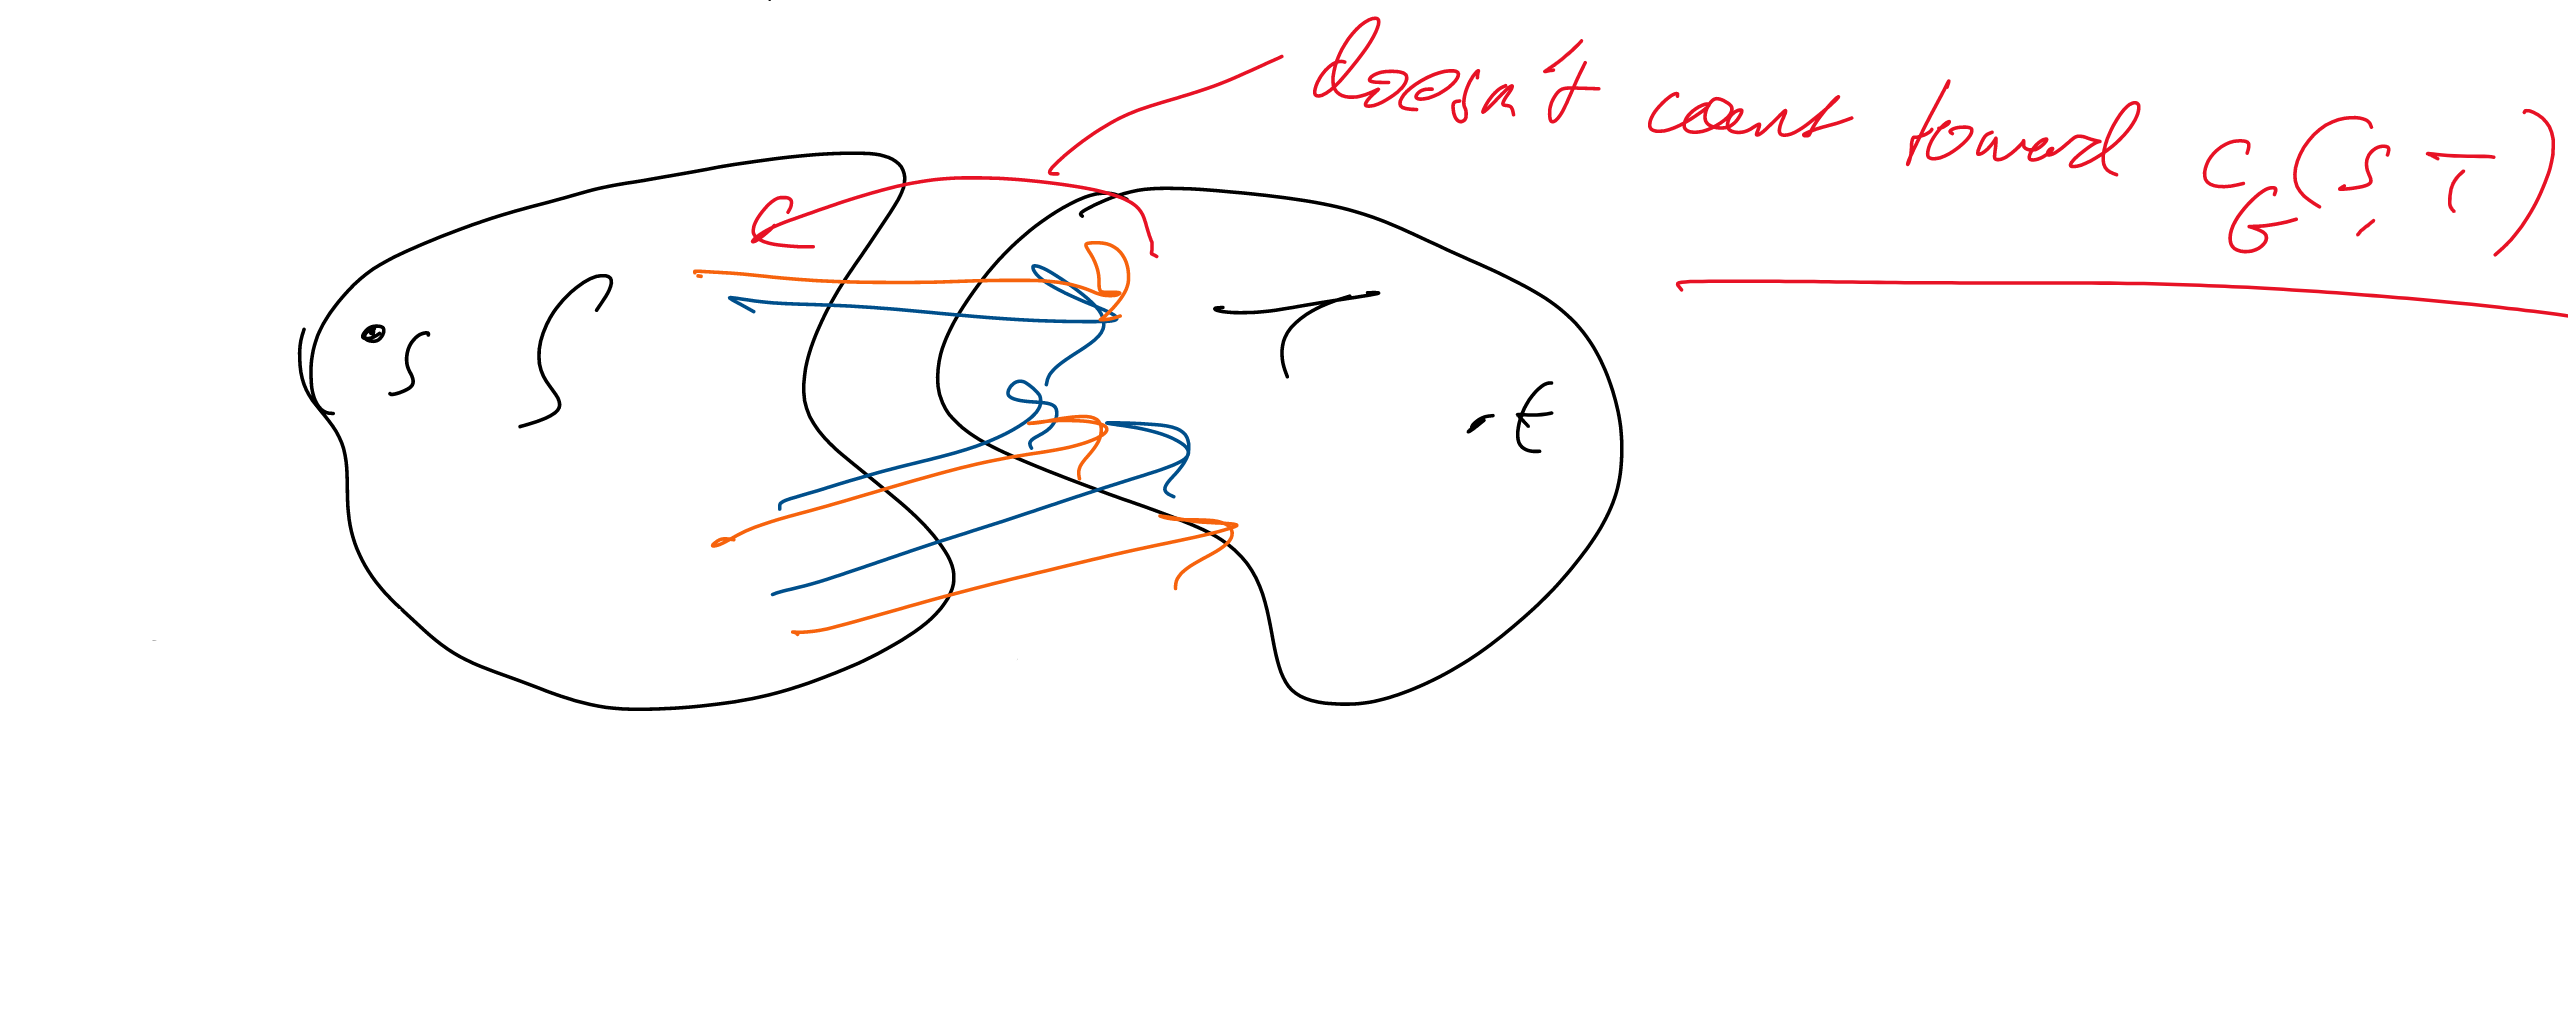
\includegraphics[width=100mm,scale=0.5]{fig/fig5_lec10.PNG}
  \caption{$s$-$t$ Cut}\label{fig:ex5}
\end{figure}
Note that the edges from $T$ to $S$ do not count towards the cut. The above equation holds for all flows with all $s$-$t$ cuts. This implies that
    $\textbf{max flow} \leq \textbf{min cut}$.
\end{proof}
This theorem is an instance of a general pattern, known as \emph{weak
duality}. Weak duality is a relationship between two optimization programs, a maximization
problem and a minimization problem, where any solution to the former has
its value upper bounded by the value of any solution to the latter.


%\newpage

\section{Algorithms for Max flow}
\paragraph{How can we find a good flow?}\ \newline

\begin{algorithm}[H]
\caption{A first attempt -- bad idea?}
\SetAlgoLined

 \(\ff \leftarrow \veczero\)\;
 \Repeat{
  Find an $s$-$t$ path flow \(\fftil\) that is feasible with respect to \(\cc - \ff\).\\
  \(\ff  \leftarrow \ff + \fftil\)}
\end{algorithm}

\paragraph{Does Algorithm 1 work?}
Consider the graph below with directed edges with capacities 1 at
every edge.
If we make a single path update as shown by the orange lines in
Figure~\ref{fig:ex6}, then afterwards, using the remaining capacity,
there's no path flow we can route, as shown in Figure~\ref{fig:ex6}.
But the max flow is 2, as shown by the flow on orange edges in
Figure~\ref{fig:ex8}.
So, the above algorithm does not always find a maximum flow: It can
get stuck at a point where it cannot make progress despite not having
reached the maximum value.
\begin{figure}[H]
  \centering
  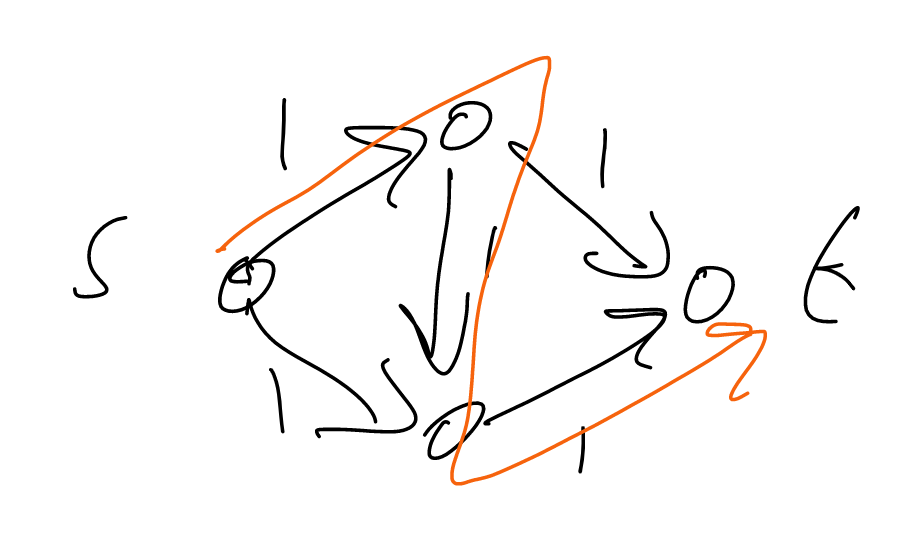
\includegraphics[width=80mm,scale=0.5]{fig/fig6_lec10.PNG}
  \caption{Sending a unit $s$-$t$ path flow through the graph.}
    \label{fig:ex6}
\end{figure}
\begin{figure}[H]
\centering
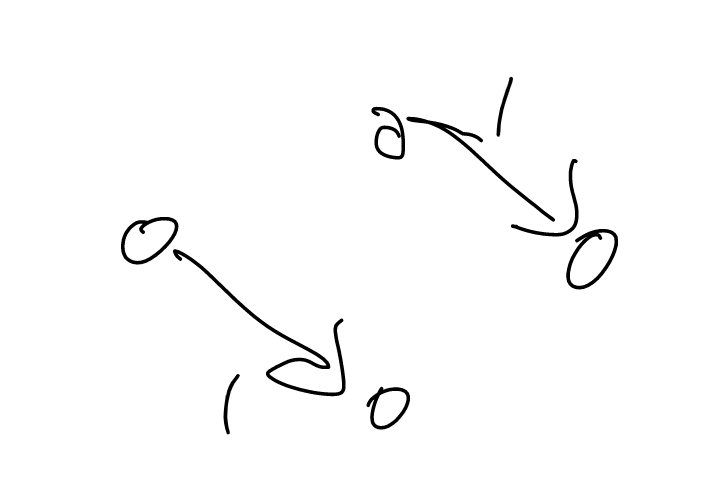
\includegraphics[width=50mm,scale=0.5]{fig/fig7_lec10.PNG}
  \caption{Remaining edge capacities after sending a path flow through
    the graph as depicted in Figure~\ref{fig:ex6}.}
  \label{fig:ex7}
\end{figure}
\begin{figure}[H]
 \centering
 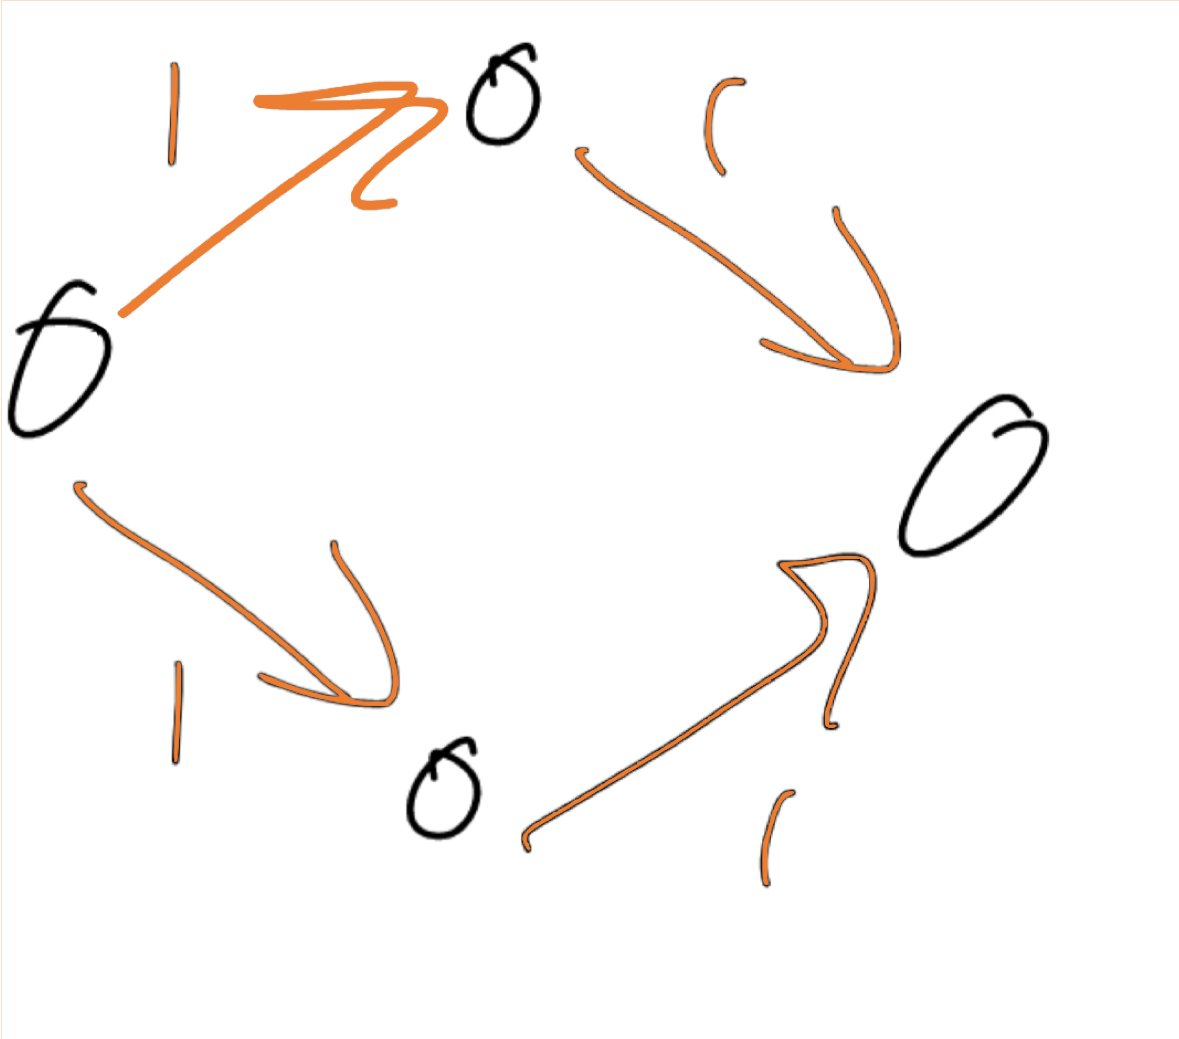
\includegraphics[width=50mm,scale=0.5]{fig/fig8_lec10.PNG}
 \caption{The flow depicted routes two units from $s$ to $t$.}
  \label{fig:ex8}
\end{figure}

\paragraph{A better approach.} It turns out we can fix the problem
with the previous algorithm using a simple fix. This idea is known as
\emph{residual graphs}.

\begin{algorithm}[H]
\SetAlgoLined
 \(\ff \leftarrow \veczero\)\;
 \Repeat{
 Find an $s$-$t$ path flow \(\fftil\) that is feasible with respect to \( - \ff\leq \fftil \leq \cc - \ff\).\\
  \(\ff  \leftarrow \ff + \fftil\)}
 \caption{Better Idea (Residual Graph)}
\end{algorithm}

The \(-\ff(e)\) can be treated as an edge going in the other direction with
capacity \(\ff(e)\).
By convention, an edge in $G$ with $\ff(e) = \cc(e)$ is called
\emph{saturated}, and we do not include the edge in $G_f$.
The graph defined above with such
capacities is called \textbf{the residual graph of \(\ff\)},
\(G_{\ff}\).  \(G_{\ff}\) is only defined for feasible \(\ff\), since
otherwise the constraint $\fftil \leq \cc - \ff$ gives trouble.


Suppose we start with a graph having a single edge with capacity 2 and we introduce a flow of 1 unit.
\begin{figure}[H]
 \centering
  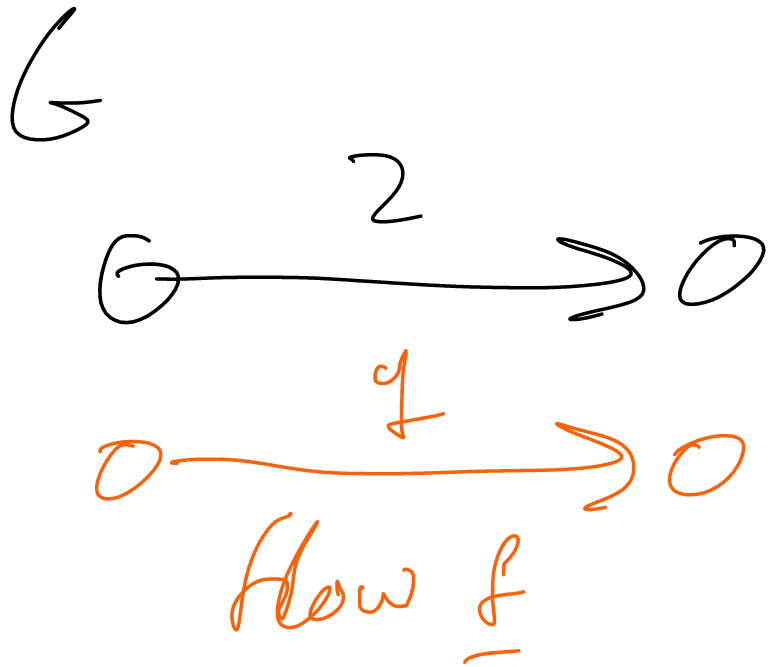
\includegraphics[width=25mm,scale=0.6]{fig/fig9_lec10.PNG}
  \label{fig:ex9}
\end{figure}
The residual graph \(G_{\ff}\) has an edge with capacity 1 going
forward and $-1$ capacity going forward, but we can treat the latter as $+1$
capacity going backwards. So it is an edge that allows you to undo the choice made to send flow along that direction.
\begin{figure}[H]
 \centering
  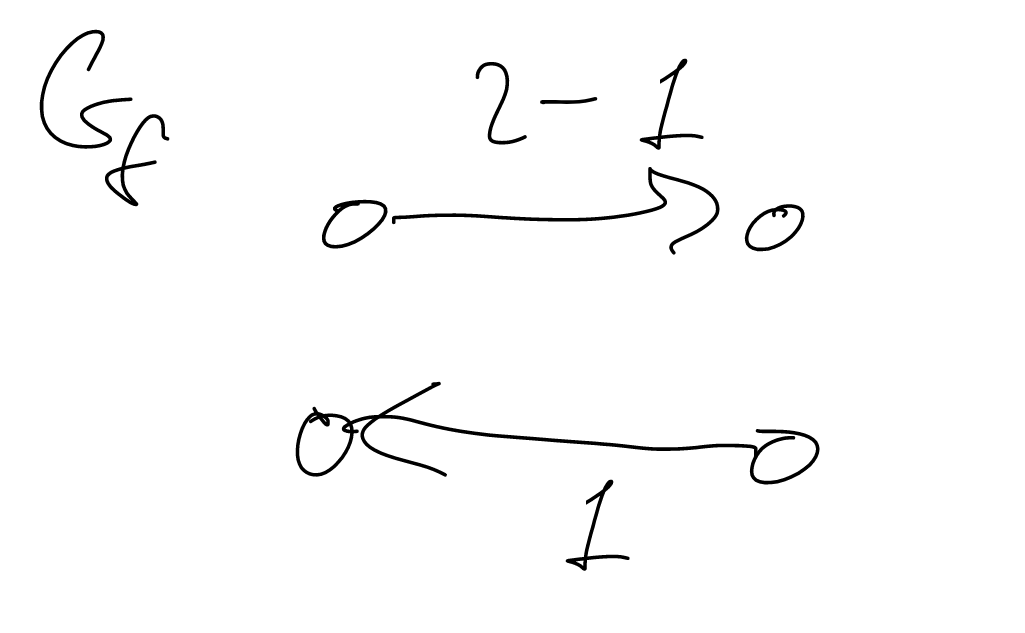
\includegraphics[width=40mm,scale=0.5]{fig/fig10_lec10.PNG}
  \label{fig:ex10}
\end{figure}
Let us consider the same example with its residual graph. The original graph is shown in Figure \ref{fig:ex11}.
\begin{figure}[H]
 \centering
  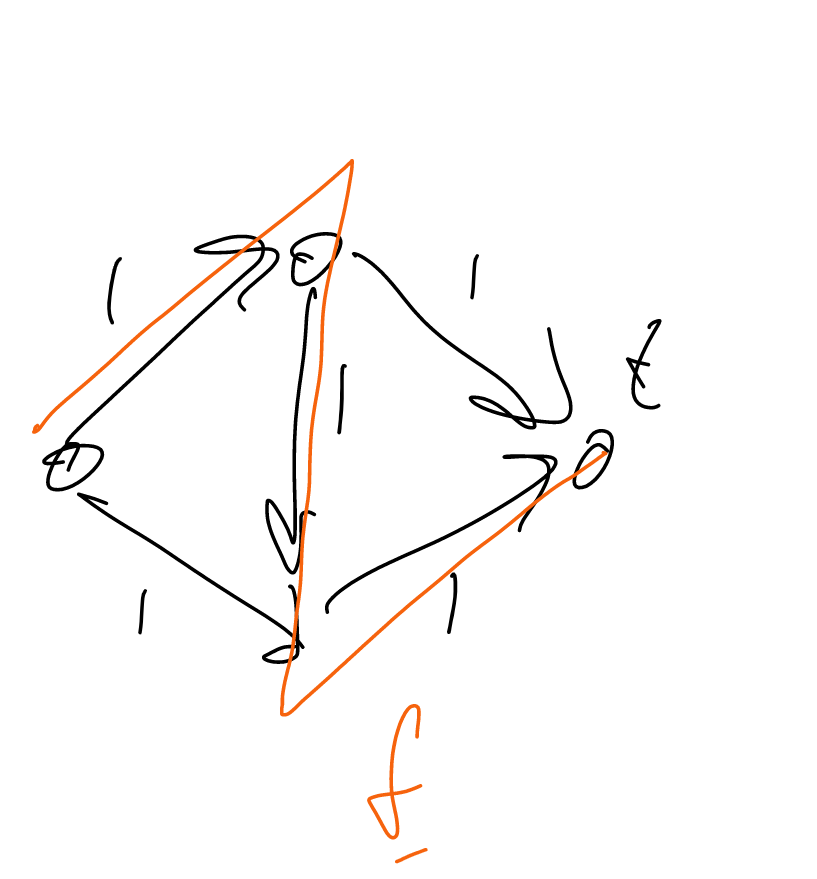
\includegraphics[width=40mm,scale=0.5]{fig/fig11_lec10.PNG}
  \caption{Original graph $G$ and an $s$-$t$ path flow in $G$ shown in
    orange.}
  \label{fig:ex11}
\end{figure}
The residual graph for the same is shown in \autoref{fig:ex12}.
\begin{figure}[H]
 \centering
  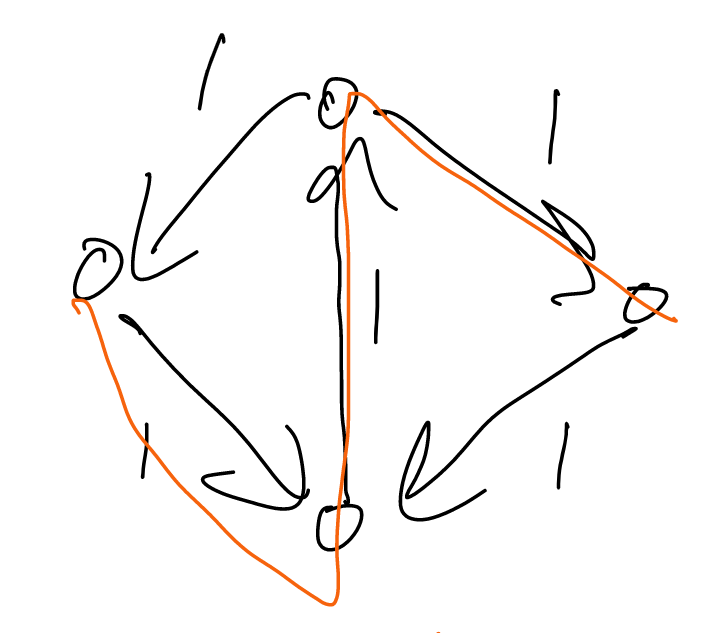
\includegraphics[width=40mm,scale=0.5]{fig/fig12_lec10.PNG}
  \caption{The residual graph w.r.t.\ the flow from
    Figure~\ref{fig:ex11}, and new $s$-$t$ path flow which is feasible
  in the residual graph.}\label{fig:ex12}
\end{figure}
Adding both flows together, we get the paths as shown in Figure \ref{fig:ex13} with value 2, which is the optimum.
\begin{figure}[H]
 \centering
  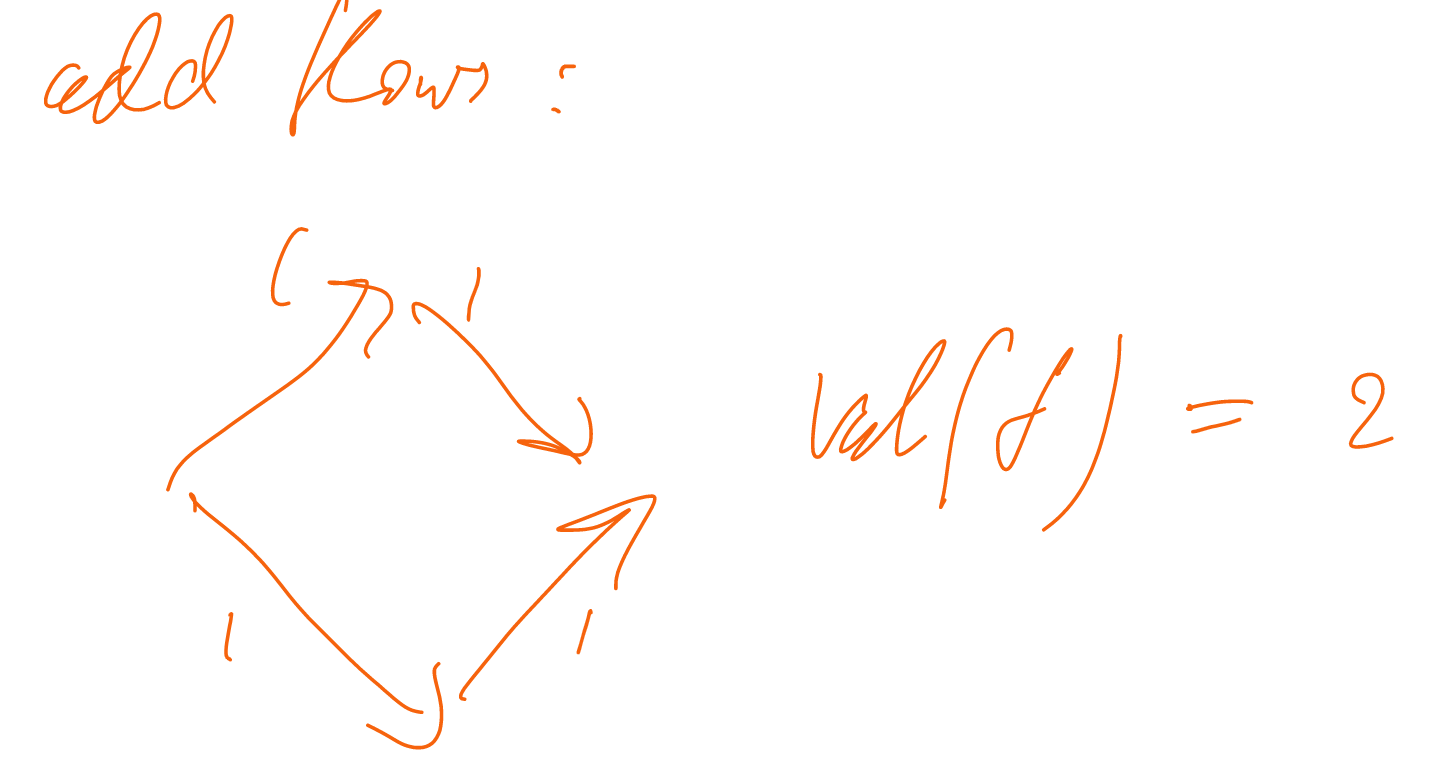
\includegraphics[width=90mm,scale=0.5]{fig/fig13_lec10.PNG}
  \caption{Maximum flow in the graph.}\label{fig:ex13}
\end{figure}
Let's prove some important properties of residual graphs.
\begin{lemma}
    \label{lem:gtogres}
Suppose   \(\ff\), \(\ffhat\) are feasible in $G$. Then this implies that \(\ffhat - \ff\)  (where negative entries count as flow in opposite direction) is feasible in \(G_{\ff}\).
\end{lemma}
\begin{proof}
\(\veczero \leq \ff \leq \cc\) and  \(\veczero \leq \fftil \leq \cc\), this implies \(-\ff \leq \fftil - \ff \leq \cc - \ff \). Hence, proved.
\end{proof}
\begin{lemma}
  \label{lem:grestog}
Suppose that \(\ff\) is feasible in \(G\) and \(\ffhat\) is feasible in \(G_{\ff}\). Then, \(\ff + \ffhat\) is feasible in G.
\end{lemma}
\begin{proof}
\(\veczero \leq \ff \leq \cc\) and  \(\ff \leq \fftil \leq \cc - \ff \), this implies \(\veczero \leq \fftil + \ff \leq \cc\).
\end{proof}

\begin{lemma}
A feasible \(\ff\) is optimal if and only if \(t\) is not reachable from \(s\) in \(G_{\ff}\).
\end{lemma}
\begin{proof}
 Let \(\ff\) be optimal, and suppose $t$ is reachable from $s$ in \(G_{\ff}\)
 then, we can find a $s$-$t$ path flow \(\fftil\) that is feasible in \(G_{\ff}\),
 and \(\val(\ff + \fftil) > \val(\ff)\). \(\ff +
 \fftil\) is feasible in $G$ by Lemma~\ref{lem:grestog}. This is a
 contradiction, as we assumed \(\ff\) was supposed to be optimal.

 Suppose $t$ is not reachable from $s$ in \(G_{\ff}\), and \(\ff\) is
 feasible, but not optimal. Let \(\ff^*\) be optimal, then by
 Lemma~\ref{lem:gtogres}, the flow \(\ff^*-\ff\) is feasible in \(G_{\ff}\) and \(\val(\ff^* - \ff) > 0\). So there exists a $s$-$t$ path flow from $s$ to $t$ in \(G_{\ff}\) (as we can do a path decomposition of \(\ff^* - \ff\)). But, this is a contradiction as $t$ is not reachable from $s$ in \(G_{\ff}\).
\end{proof}

\begin{theorem}[Max Flow $=$ Min Cut theorem] The maximum flow in a directed graph G equals the minimum cut.
\end{theorem}
\begin{proof}
%\subsubsection{Strong Duality}
Consider the set $S = \setof{ \text{vertices reachable from } s \text{ in
  } G_{\ff}}$.
Note that \(\ff\) saturates the
edge capacities in cut \(S,V\setminus S\) in G:
Consider any edge from $S$ to $T:=V \setminus S$ in $G$. Since this edge does not
exist in the residual graph, we must have $\ff(e) = \cc(e)$.
% Suppose for a contradiction that say that there exists an edge from set $S$ to set $T$ in G as shown in Figure~\ref{fig:ex13} below. Since $S$ and $T$ are disconnected in \(G_{\ff}\), it means that the edges in G from $S$ to $T$ should have used up all their capacity.
\begin{figure}[H]
 \centering
 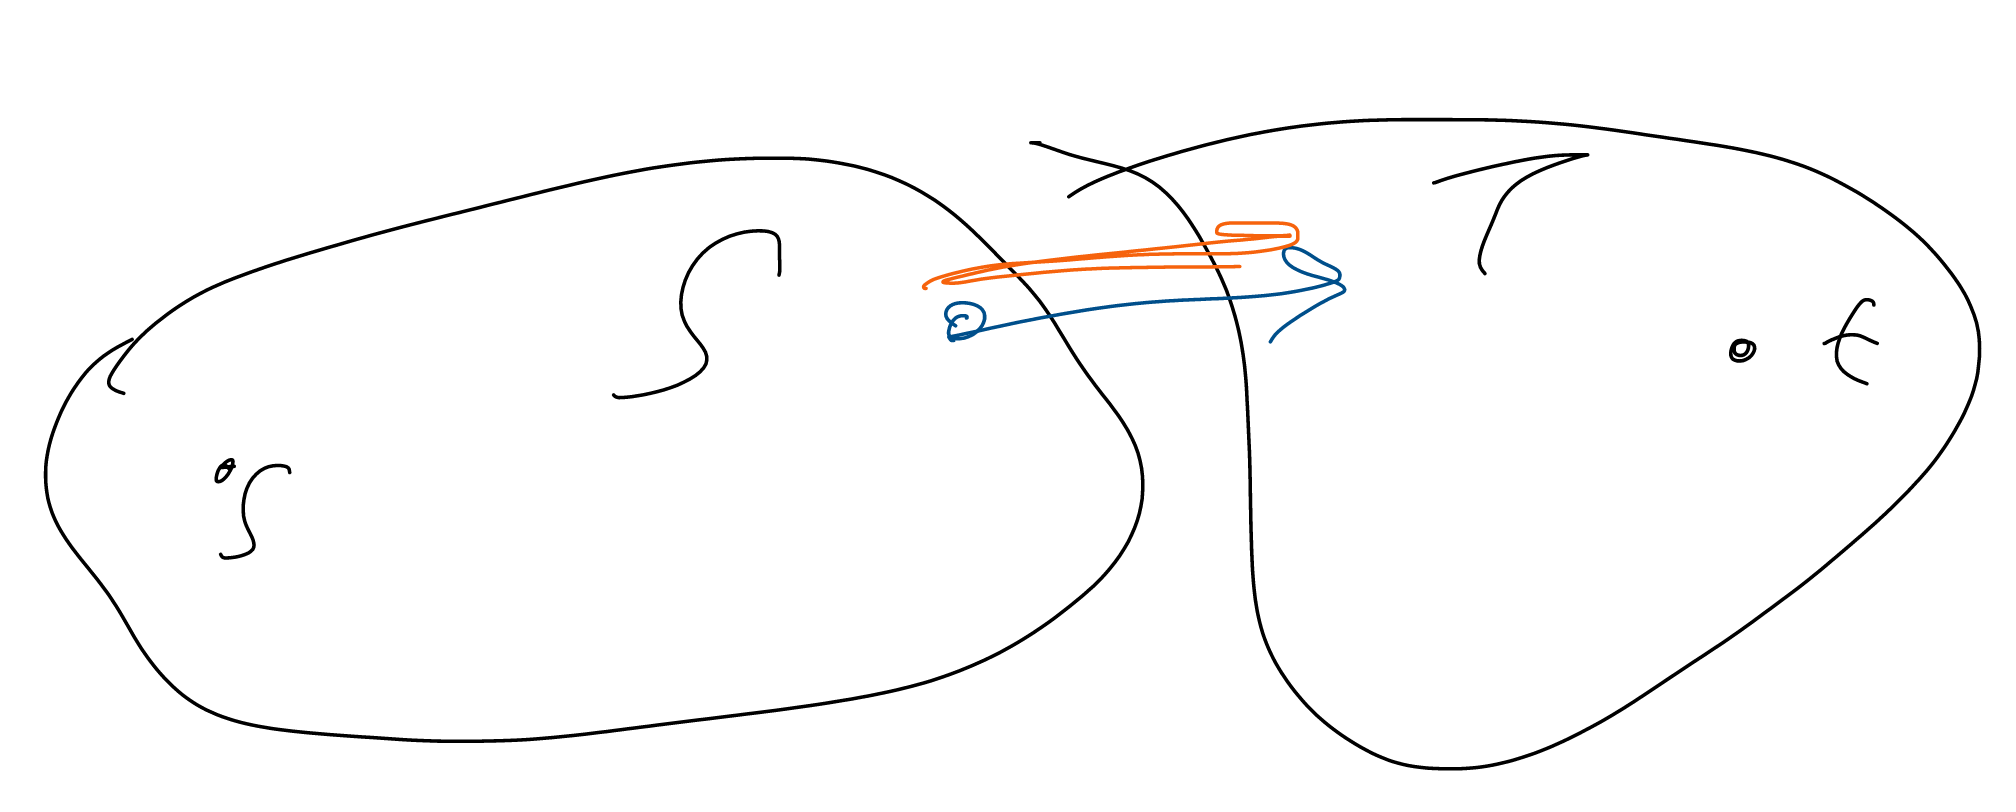
\includegraphics[width=60mm,scale=0.5]{fig/fig14_lec10.PNG}
 \caption{The cut between vertices reachable from $S$ and everything
   else in $G_f$ must have all outgoing edges saturated by $\ff$.}
  \label{fig:ex14}
\end{figure}
%
This means that
\begin{equation} \nonumber
   \val(\ff) \geq c_G(S, V \setminus S).
\end{equation}
Since we already know the opposite inequality by weak duality, we have
shown that
\begin{equation} \nonumber
   \val(\ff) = c_G(S, V \setminus S)
\end{equation}
which proves the \textbf{Max Flow} = \textbf{Min Cut} theorem; also called strong duality.
\end{proof}

\begin{remark}
  Note that this proof also gives an algorithm to compute an $s,t$-min
  cut given an $s,t$ maximum flow: Take one side of the cut to be the
  set $S$ of nodes reachable from $s$ w.r.t. the 
\end{remark}

\paragraph{Ford-Fulkerson Algorithm.}\ \\
\begin{algorithm}[H]
\SetAlgoLined
 \Repeat{
 Add update by arbitrary $s$-$t$ path flow in \(G_{\ff}\) (augment the flow \(\ff\) by the path flow)
}
 \caption{Ford-Fulkerson Algorithm}
\end{algorithm}


\subsubsection{Convergence properties and analysis of runtime of Ford-Fulkerson algorithm}
\begin{itemize}
    \item \textbf{Does this algorithm terminate?}\\
    The algorithm terminates if the capacities are integers. However for irrational capacities the algorithm may not terminate.
    \item \textbf{Does it converge towards the max flow value?}\\
    No, it does not converge to max flow value if the updates are poor and the capacities are irrational.
\end{itemize}

\begin{lemma}
Consider Ford-Fulkerson algorithm with integer capacities. The algorithm terminates in \(\val(\ff^*)\) augmentations i.e.\ $O(m \val(\ff^*))$ time.
\end{lemma}
\begin{proof}
Each iteration increases the flow by at least one unit as the
capacities in \(G_{\ff}\) are integral and each iteration can be
computed in  $O(m)$ time.
\end{proof}

\paragraph{Can we do better than this?}
Suppose we pick the maximum bottleneck capacity (minimum capacity
along path) augmenting path. This gives an algorithm that is better in
some regimes.

How to pick the maximum bottleneck capacity augmenting path? We are
going to perform a binary search on the capacities in \(G_{\ff}\), to
find a path with maximum bottleneck capacity.
Each time our binary search has picked a threshold capacity, we then
try to find an $s$-$t$ path flow in \(G_{\ff}\) using only  edges with
capacity above that threshold. If we find a path, the binary search
tries a higher capacity next. If we don't find a path, the binary search
tries a lower capacity next.

Using this approach, the time to find a single path is $O(m \log(n))$ where $m$ is number of edges in the graph.
This path must carry at least a \( \frac{1}{m}\) fraction of the total
amount of flow left in \(G_{\ff}\). For instance, if \(\hat{F}\) is
the amount of flow left in \(G_{\ff}\), then the path must carry
\(\frac{\hat{F}}{m}\) flow (from the path decomposition lemma, there
are at most $m$ paths, and the one carrying the most flow must carry
at least the average amount).

So if the flow is integral, the algorithms completes when
\begin{equation}\nonumber
    \left( 1 - \frac{1}{m}\right)^T \val(\ff^*) < 1
\end{equation}
where $T$ is the number of augmentations.

This means
\begin{equation}\nonumber
    T = m \log{F}
\end{equation}
\begin{align*}
\text{Total time} &= O(m \log{n} T) \\
                  &= O(m^2 \log{n} \log{F})\\
                  &\leq O(m^2 \log{n} \log{mU}) \text { as }  F \leq m U \text{ where U is the maximum capacity}\\
\end{align*}

\paragraph{Current state-of-the-art approaches for Max Flow.} For the
interested reader, we'll briefly mention the current state-of-the-art
for Maximum Flow algorithms, which is a  very active area of research.
% TODO(Tim): Would be nice to provide references here..
\begin{itemize}
   \item In undirected graphs, there are algorithms known which
     compute a $(1+\epsilon)$-approximate solution in time
     $\tilde{O}(m/\epsilon)$ \cite{S17}.
    \item Strongly polynomial time algorithm:
     \begin{itemize}
       \item has to work with real valued capacities, then the best time $O(mn)$ by Orlin.
    \end{itemize}
    \item Restricted to unit capacities:
    \begin{itemize}
        \item Old algorithm that runs in \(O(m^{1.5})\).
        \item The time for this was improved in 2014 to
          \(O(m^{\frac{10}{7}} )\) by Madry.
        \item Run time improved again in 2020 to \(\tilde{O}(m^{\frac{4}{3}})\) by Liu and Sidford.
    \end{itemize}
  \item General integer capacities: For a long time, the
    state-of-the-art was a result by Goldberg and Rao achieving a
    runtime of \(O(m \min(\sqrt{m},n^{2/3}) \log(n) \log(U) )\) where $U$ is the
    maximum capacity.
    In dense graphs, the best running time is now $\tilde{O}(m +
    n^{3/2})$ \cite{BLLSSSW21}, and in sparse graphs, a recently
    accounted result makes a small improvement over Goldberg-Rao,
    achieving a running time of  \(O(m^{3/2 - 1/328} \log(n) \log(U) )\) where $U$ is the
    maximum capacity \cite{GLP21}.
\end{itemize}
%\end{document}


% % Consider the flow for the graph shown in Figure (\ref{fig:ex3}). Once we have chosen the flow along the green paths, there is no other way to update the flow without violating the capacity constraints. The value that this flow routes is 2. However, this is not the optimal flow. As can be seen from Figure (\ref{fig:ex4}), the value of optimal flow is 3.\\

% \begin{figure}[h!]
%  \centering
%   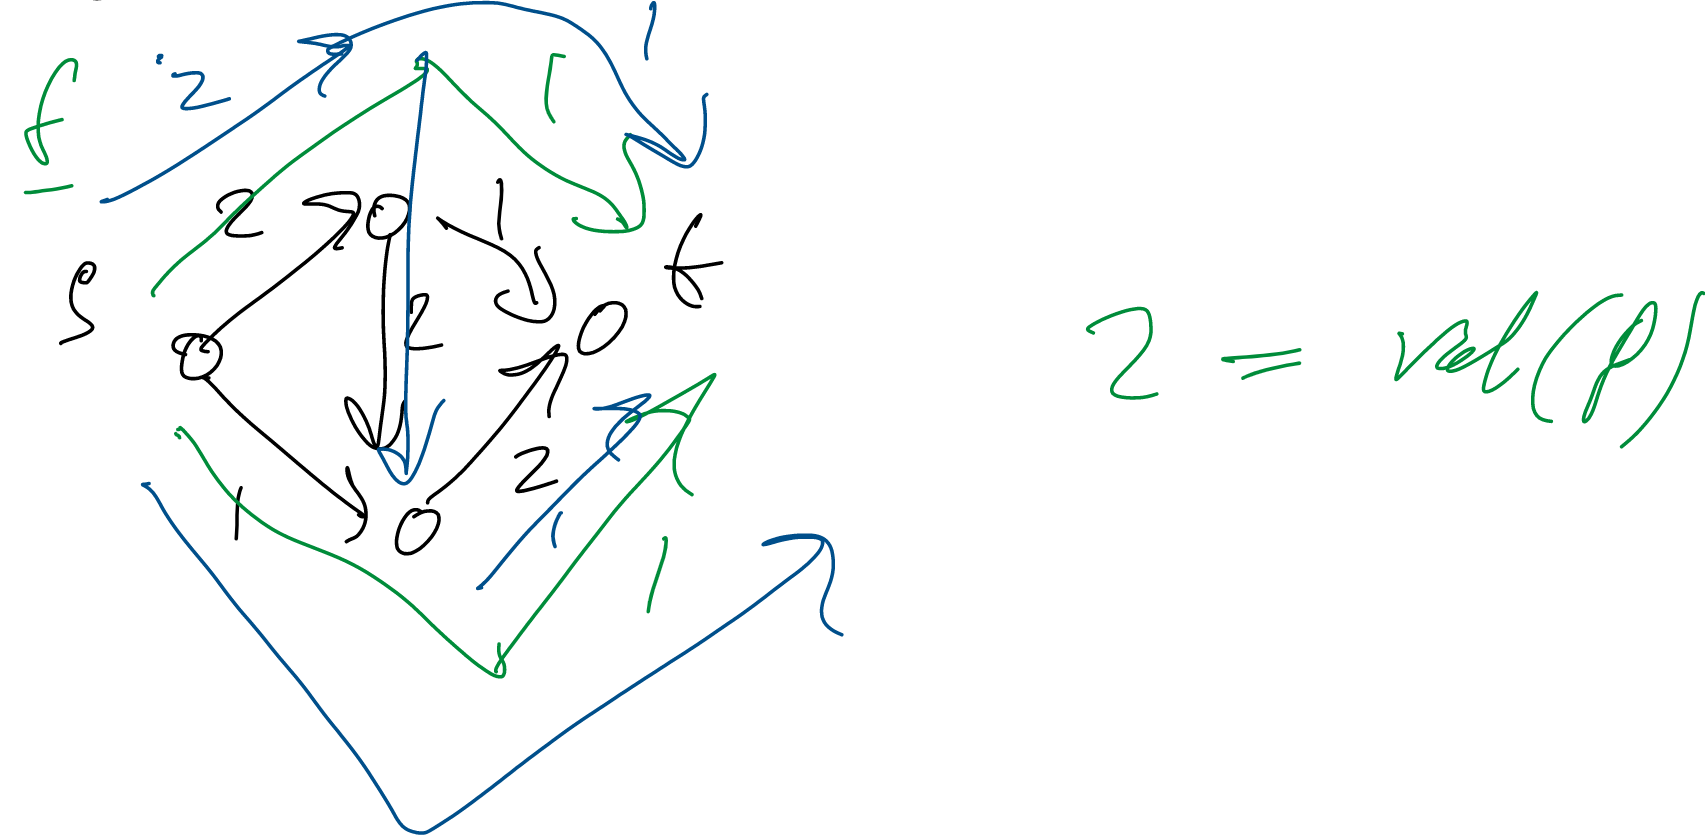
\includegraphics[width=70mm,scale=0.1]{fig/fig3_lec10.PNG}
%   \caption{Flow on Diamond graph}
%   \label{fig:ex3}
% \end{figure}


% \begin{figure}[h!]
%  \centering
%   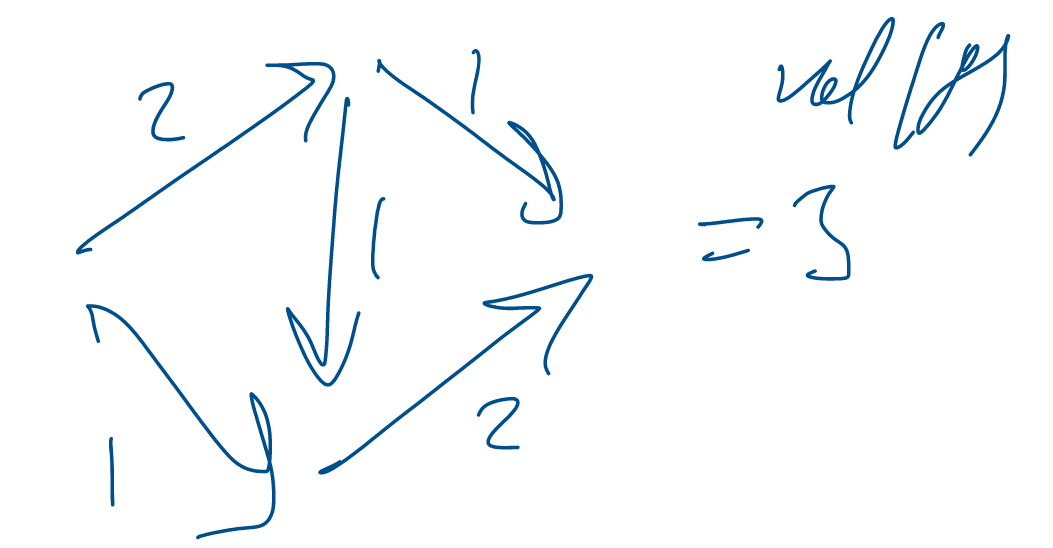
\includegraphics[width=70mm,scale=0.1]{fig/fig4_lec10.PNG}
%   \caption{Optimal flow on Diamond graph }
%   \label{fig:ex4}
% \end{figure}


%%% Local Variables:
%%% mode: latex
%%% TeX-master: "agao21_script"
%%% TeX-engine: luatex
%%% End: